\chapter{Analysis of the ported \textsc{BaseX} Android version}
\label{cha:analysis}
The following chapter outlines how the migrated \textsc{BaseX} Android database is analyzed.
The focus at this part lies on the evaluation and the performance of the library.
First the specification of the test devices is outlined and an estimation is made to show how the performance of the various devices differ.
Therefore different benchmarks has been executed to approximate the distinctive hardware properties and their execution times.
In the next chapter is shown that the migrated database works without errors and failures on the Android mobile platform using a real devices.
For this purpose different unit test has been also migrated to test the functionality.
After evaluation the functionality the performance has been investigated.
An overview of the performance an XML benchmark set, which is especially designed to test the performance of XQuery executions, has been used.
\section{Evaluation of the test devices}
\label{sec:evaluation-of-the-test-devices}
For the measurement of the performance two devices are being used.
First, for testing the \textsc{BaseX} mobile version an Android Tablet PC Samsung Galaxy Tab 2 10.1 and for the normal \textsc{BaseX} version a Lenovo Thinkpad laptop have been used.
Their technical specifications can be seen in Table\ref{tab:test-dev-specs}.
\begin {table}[htpb] 
  \centering
\begin {tabular} {|r|r|r|r|r|r|}
  	\hline
	&CPU&RAM&filesystem&operating system\\
	\hline
	Laptop&Intel Core2 Duo CPU L7100&2 Gb&ext4&Arch Linux\\
	&1.2 GHz&&&(3.12.0)\\
	\hline
	Tablet&Dual-core Cortex-A9&1 Gb&ext4&Android\\
	&1 GHz&&&(4.0.3)\\
	\hline
\end {tabular}
\caption {The technical specifications of the two devices, used for benchmark testing.}
\label {tab:test-dev-specs}
\end {table}

Looking at this table it can be seen that the only similarity of both systems is that they are using the same filesystem, which is ext4, which is short for fourth extended filesystem.
The RAM of the laptop is the double amount of the tablet available RAM and both devices have a dual core CPU with around 1 GHz.
Even if the specifications are not so much differ on the first look, their performance varies in some factors.
Therefore a measurement of the input/output (IO) and CPU speed of booth devices has been made in Section~\ref{sec:evaluation-of-the-test-devices} to get a clearer look how the devices differ.


%\section{Evaluating the working \textsc{BaseX} Android port}
%\label{sec:evaluating-the-working-basex-android-port}
%\textbf{TODO}\\
%In this section will be shown that the created \textsc{BaseX} Android port works and fit all requirements.
%For this purpose the given JUnit tests were been migrated to Android too.
%This shows that all functions work like they work on the standard Java version.
The two devices which have been used to benchmark \textsc{BaseX} are totally different and not just in the fact that one is laptop and the other a tablet PC.
They differ in many hardware aspects, but there are two different factors, that are interesting to identify a systems speed and are used for the given purpose.
These are the CPU speed and the input/output (IO) speed, where IO speed is a headline for different operations.
Broadly speaking it can be said that the IO speed can be divided into read and write operations.\\
To measure this values the benchmark tool Bonnie++\footnote{\url{http://www.coker.com.au/Bonnie++/}} is used.
This tool executes different operations and measures how many of these operations can be executed in one second.
It tests sequential output, sequential input, random seeks, sequential create and random create.\\
The sequential output represents the write speed of the system, Bonnie++ uses three different methods to measure this value.
First it writes one character after another by using the \textit{putc()} systemcall. 
After this operation it writes whole blocks with the size of 8192 bytes by using the write() systemcall and than calling the close() systemcall.
The last test in this category is the rewrite test and differs from the write test, that the file is not closed after writing.
Therefore one block write comply with 8192 \textit{putc} calls and is way more effective and faster than writing single characters.
The next test is to measure the random seek operations per seconds, which means how often the read/write position can be changed.
It also measures the latency which represents the rotation speed of the disk, but this is obsolete because both systems have flash storage and so there is no revolution per minute to measure.
Bonny is written in C++ and is available on most Linux distributions, but to use it on Android it is necessary to build it from its sources by using the, in Chapter~\ref{sec:migration:the-android-project-structure} mentioned, Android Native Development Kit (NDK).
This provides a cross compiler which makes it possible to build C++ code for Android.
For the execution of the benchmarks the version 1.96 from Bonnie++ has been used.
The results of these test executions can be seen in table~\ref{tab:bonnie-results-out}.
%\begin {table}
%\begin {tabular} {|r|r|r|r|r|r|r|r|r|r|r|r|r|}
%	\hline
%		&\multicolumn {3} {|c|} {Sequential}&\multicolumn {2} {|c|} {Sequential}&Random&\multicolumn {3} {|c|} {Sequential}&\multicolumn {3} {|c|} {Random}\\
%		&\multicolumn {3} {|c|} {Output}&\multicolumn {2} {|c|} {Input}&Seeks&\multicolumn {3} {|c|} {Create}&\multicolumn {3} {|c|} {Create}\\
%	\hline
%		&K/sec&K/sec&K/sec&K/sec&/sec&/sec&/sec&/sec&/sec&/sec&/sec&/sec\\
%	\hline
%	Laptop&201&62180&23850&907&98239&1161&17134&137752&13032&19442&170028&11774\\
%	\hline
%	Tablet&5&20828&8756&596&23768&475.6&39&361&167&42&391&238\\
%	\hline
%	\hline
%	Factors&40.20&2.99&2.72&1.52&4.13&2.44&439.33&381.58&78.04&462.90&434.85&49.47\\
%	\hline
%\end {tabular}
%\caption {Results of the Bonnie++ benchmarks.}
%\label {tab:bonnie-results}
%\end {table}


\begin {table}[htpb] 
  \centering
\begin {tabular} {|r|r|r|r|r|r|r|}
	\hline
		&\multicolumn {3} {|c|} {Sequential}&\multicolumn {2} {|c|} {Sequential}&\multicolumn {1} {|c|}{Random}\\
		&\multicolumn {3} {|c|} {Output}&\multicolumn {2} {|c|} {Input}&\multicolumn {1} {|c|}{Seeks}\\
	\hline
		&Char&Block&Rewrite&Char&Block&\\
	\hline
	Laptop&201K&62180K&23850K&907K&98239K&1161\\
	\hline
	Tablet&5K&20828K&8756K&596K&23768K&475.6\\
	\hline
	\hline
	Factors&40.20&2.99&2.72&1.52&4.13&2.44\\
	\hline
\end {tabular}
\caption {Results of the Bonnie++ in- and output benchmarks.}
\label {tab:bonnie-results-out}
\end {table}


Bonnie++ also measures the sequential and random create of a file.
Therefore it creates, queries its status and deletes a file by using the Posix systemcalls \textit{creat()}, \textit{stat()} and \textit{unlink()}.
The results of this test can be seen in Table~\ref{tab:bonnie-results-create}
\begin {table}[htpb] 
  \centering
\begin {tabular} {|r|r|r|r|r|r|r|}
	\hline
		&\multicolumn {3} {|c|} {Sequential}&\multicolumn {3} {|c|} {Random}\\
		&\multicolumn {3} {|c|} {Create}&\multicolumn {3} {|c|} {Create}\\
	\hline
		&creat()&stat()&unlink()&creat()&stat()&unlink()\\
	\hline
	Laptop&17134&137752&13032&19442&170028&11774\\
	\hline
	Tablet&39&361&167&42&391&238\\
	\hline
	\hline
	Factors&439.33&381.58&78.04&462.90&434.85&49.47\\
	\hline
\end {tabular}
\caption {Results of the Bonnie++ sequential/random create benchmarks.}
\label {tab:bonnie-results-create}
\end {table}


%\begin {table}
%\begin {tabular} {|r|r|r|r|r|r|r|}
%	\hline
%		&\multicolumn {3} {|c|} {Sequential}&\multicolumn {2} {|c|} {Sequential}&\multicolumn {1} {|c|}{Random}\\
%		&\multicolumn {3} {|c|} {Output}&\multicolumn {2} {|c|} {Input}&\multicolumn {1} {|c|}{Seeks}\\
%	\hline
%		&Char&Block&Rewrite&Char&Block&\\
%	\hline
%	Laptop (per seconds)&201K&62180K&23850K&907K&98239&1161\\
%	\hline
%	Tablet (per seconds)&5K&20828K&8756K&596&23768K&475.6\\
%	\hline
%	\hline
%	Factors&40.20&2.99&2.72&1.52&4.13&2.44\\
%	\hline
%\end {tabular}
%\caption {Results of the Bonnie++ benchmarks.}
%\label {tab:bonnie-results}
%\end {table}


By analyzing these values it can be said that the laptop is overall faster than the tablet PC.
It is well known that IO operations are the most expensive one on Android, so the achieved result is no surprise. 
But with these values it can be said that there are factors which can tell how much faster it is in specific operations.
This factors are impossible to optimize, because they are a hardware constraint and only changing the hardware can improve them, but they are still important to identify the bottlenecks of the mobile \textsc{BaseX} version.\\
Analyzing Table~\ref{tab:bonnie-results-create} and having a look at the factors shows one value which is, compared to the other factors, extremely high.
The sequential write per character is 40 times faster on the laptop than on the tablet, considering this, it is clear to avoid writing by character instead by block.
Writing by using the block mechanism is just three times slower on the tablet.
The sequential reading of a single character is at the tablet just 1.52 times slower than the at the notebook.
Though the factor of the block reading is quite higher than the character reading factor it is sure to use the block reading because it is much faster than character reading.
But by using block reading the factor need also be considered in the \textsc{BaseX} benchmarks later in chapter~\ref{sec:analysing-the-execution-performance}.
\\
Looking at Table~\ref{tab:bonnie-results-create} it can be seen that the sequential/random creation, reading and deleting is very slow on the Android devices compared to the laptop.
Considering this it should be avoided to often create files, because this is very slow.\\
Bonnie++ gives a good overview about how fast the two system handle their IO operations and how they differ in this aspect.
But there is also another factor which affects the speed of the execution of a program.
This is the CPU speed, it is obvious that this also differs on both test devices.
To evaluate the CPU times a Java program has been written which executes four different CPU intensive operations.
First it does the naive factorial of 5000, where naive means that it just iterates till 5000 and multiplies every step to the result.
The second test is a recursive calculation of the 100th Fibonacci number.
The third sorts an ascending ordered array of 10000 items using the bubble-sort algorithm.
This is done because this is the worst case for the bubble-sort algorithm and has a complexity of $\mathcal O(n^2)$.
The last test makes a naive test if the number 666667 is prime or not, by testing to divide the number by every candidate step by step till the candidate is the square root of the number.
All these test are very CPU intensive, because they use only arithmetic operations.
The results of these test can be seen in Table~\ref{tab:cpu-results}.
\begin {table}[htpb] 
  \centering
\begin {tabular} {|l|r|r|r|r|}
	\hline
		&Factorial&Fibonacci&Bubble Sort&Prime Number\\
	\hline
	Laptop&&&&\\
	(avg. on 1000 runs)&98.19 ms&248.63 ms&180.53 ms&15.85 ms\\
	\hline
	Tablet&&&&\\
	(avg. on 1000 runs)&491.15 ms&2336.35 ms&1045.52 ms&76.41 ms\\
	\hline
	\hline
	Factors&5&9.4&5.8&4.8\\
	\hline
\end {tabular}
\caption {Results of the CPU benchmarks.}
\label {tab:cpu-results}
\end {table}


Except the Fibonacci test it can be said that the CPU of the laptop is about five times faster than the one of the laptop.
This is like the different IO parameters a factor which could not be improved and has to be considered in the \textsc{BaseX} benchmarks as well.
These evaluation is for measuring the performance of the two \textsc{BaseX} versions and how to cope with the results achieved by two different platforms on two different devices.


\section{Analyzing the execution performance}
\label{sec:analysing-the-execution-performance}
To investigate the performance of the Android version of \textsc{BaseX} the benchmark suite \textit{XMark} has been used.
\textit{XMark} creates random XML files and has a set of twenty predefined queries that can be used to measure the execution performance of an \textit{XQuery} implementation.
It offers the possibility to choose the size of the random XML files, so that the test queries can be executed on different file sizes.
Therefore it is also being used to find the maximum supported size of a \textsc{BaseX} database on Android.


\subsection{The XMark benchmark suite}
\label{subsec:the-xmark-benchmark-suite}
The XMark benchmark suite is used to identify the speed of the \textsc{BaseX} Android version.
Therefore it offers 20 different XQueries which are designed to benchmark a XQuery implementation.
The queries are separated into different categories, where every category targets a specific aspect of query execution.
The XML files that can be generated by using XMark are all containing the same elements and every file is well-formed.
The content of the generated XML files is randomly generated by using the 17000 most frequently used words~\footnote{ignoring stop words} in the plays of Shakespeare~\cite{schmidtxmark}.
The structure of the randomly generated XML files can be seen in Figure~\ref{fig:xmark-file-structure}.
\begin{figure}[h]
\begin{center}
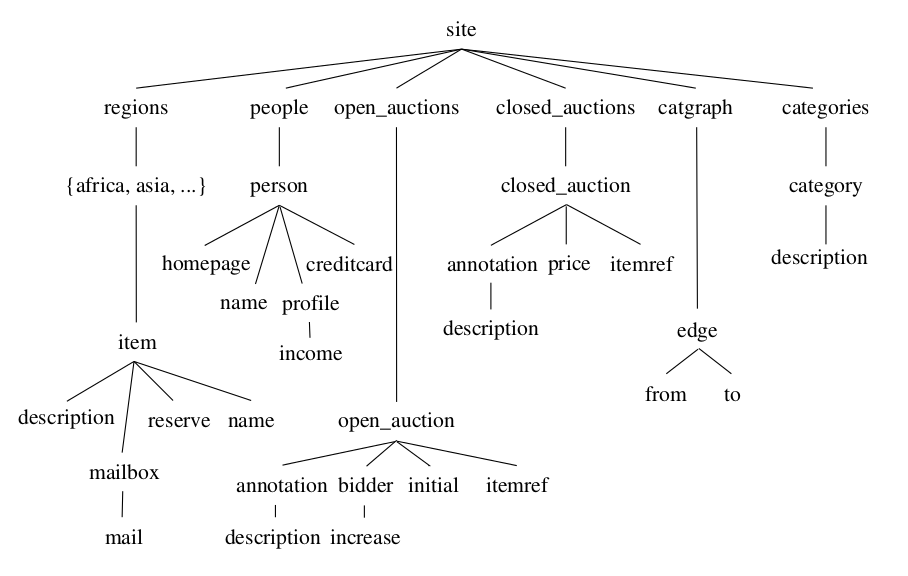
\includegraphics[scale=0.42]{images/xmark-file-elements.png} 
\caption{The structure of a generated XMark XML file. Source:\cite{schmidtxmark}}
\label{fig:xmark-file-structure}
\end{center}
\end{figure}

The size of the XML files can be chosen during the generation process of XMark.
For testing \textsc{BaseX} 15 different files were been generated.
The smallest with the size of 100 Kb followed by files with a size increasing by 100 Kb steps.
Hence, the biggest generated file has a size of 1.4 Mb.\\
The different queries can be seen in Table~\ref{tab:xmark-queries}.
\begin {table}[htpb] 
  \centering
	\begin{tabular}{r|l}
	  \hline
	  1&Return the name of the person with ID 'person0'.\\
	  \hline
	  2&Return the initial increase of all open auctions.\\
	  \hline
	  3&Return the first and current increase of all open auctions whose current\\
	  &increase is at least twice as high as the initial increase.\\
	  \hline
	  4&List the reserves of those open auctions where a certain person issued\\
	  &a bid before another person.\\
	  \hline
	  5&How many sold items cost more than 40.\\
	  \hline
	  6&How many items are listed on all continents?\\
	  \hline
	  7&How many pieces of prose are in our database?\\
	  \hline
	  8&List the names of persons and the number of items they bought.\\
	  &(Joins person, closed\_auction)\\
	  \hline
	  9&List the names of persons and the names of items they bought in Europe.\\
	  &(Joins person\_auction, item)\\
	  \hline
	  10&List all persons according to their interest; use French markup\\
	  &in the result.\\
	  \hline
	  11&For each person, list the number of items currently on sale whose\\
	  &price does not exceed 0.02\% of the person's income.\\
	  \hline
	  12&For each richer-than-average person, list the number of items currently\\
	  &on sale whose price does not exceed 0.02\% of the person's income.\\
	  \hline
	  13&List the names of items registered in Australia along with\\
	  &their description.\\
	  \hline
	  14&Return the names of all items whose description contains the word 'gold'.\\
	  \hline
	  15&Print the keywords in emphasis in annotations of closed auctions.\\
	  \hline
	  16&Return the IDs of those auctions that have one or more keywords\\
	  &in emphasis.\\
	  \hline
	  17&Which persons don't have a homepage?\\
	  \hline
	  18&Convert the currency of the reserve of all open auctions to\\
	  &another currency.\\
	  \hline
	  19&Give an alphabetically ordered list of all items along with their location.\\
	  \hline
	  20&Group customers by their income and output the cardinality of each\\
	  &group.\\
	  \hline
	\end{tabular}
	\caption {The XMark queries. Source:\cite{schmidtxmark}}
\label {tab:xmark-queries}
\end {table}


The queries are divided into various categories, which are aiming to benchmark several functionalities and concepts of XML.
Category one includes just Query 1 and tests the performance of an exact match.
The second category analyzes the behavior of the database by querying it with order constraints.
This category contains the queries 2, 3 and 4.
Casting is the purpose of the third category, which only includes Query 5.
The next category contains the queries 6 and 7, and tests the regular path expressions.
Chasing references is the topic of Category 5 that holds Query 8 and 9.
Constructing new elements and querying them is the purpose of the next category that includes only Query 10.
Benchmarking the execution of queries with a large result set by using joins is the goal of Category 7, which involves Query 11 and 12.
Query 13 is the only query in the next category, which aims to test the performance of reconstruction of a document.
Search a full text by using a key word is the purpose of Category 9 that just includes Query 14.
The next category tests the performance of deep path traversals without wildcards, this includes the Queries 15 and 16.
Category 11 includes Query 17 and investigates the performance of the database by querying missing elements.
User defined functions are the content of the next category which contains Query 18.
To investigate the performance of the database executing a query that sorts the result is the purpose of Category 13 which is achieved by Query 19.
The last category is used to test the speed of an execution of a simple aggregation by using the last query.~\cite{schmidtxmark}.

\subsection{The Results of the Benchmark Execution}
\label{sec:the-results-of-the-benchmark-execution}
To execute the XMark queries two applications have been developed, one for testing the \textsc{BaseX} desktop version and one for the Android version.
These two programs are the same except the target platform and the used \textsc{BaseX} version.
They have the same functionalities and they operate equal.
First the programs create 15 databases and add the, in the section before mentioned 15 XML files, to these databases.
After this operations the application opens one database after another and executes every XMark query on it.
Every query is executed a hundred times and the average time consumption is being calculated and stored into a file.
The result of the execution of the application using the Laptop can be seen in Figure~\ref{fig:xmark-laptop} and the result of the execution using the Tablet is shown in Figure~\ref{fig:xmark-tablet}.

\begin{figure}[!ht]
  \begin{center}
  \begin{gnuplot}[terminal=pdf, terminaloptions=color, scale=1.1]
          set title 'Laptop Steps'
	  set datafile separator ','
	  set xlabel 'Query'
	  set ylabel 'Average time in ms(100 executions)'
	  set xrange [0:21]
	  set xtics 1,1,20
	  set logscale y
	  set grid ytics lt 0 lw 1 lc rgb '#bbbbbb'
	  set grid xtics lt 0 lw 1 lc rgb '#bbbbbb'
	  set key samplen 2 spacing .5 font ',8'
	  show grid
	  set style fill solid 0.8 border -1
	  set boxwidth 0.5 relative
	  plot for [i=1:14] 'benchmarks/basex-steps-laptop-transposed.csv' u ($0+1):i title ''.i.'00kb' with linespoints
	\end{gnuplot}              
	\caption{The results of the XMark benchmark queries executed on the Laptop.}
	\label{fig:xmark-laptop}
	\end{center}
\end{figure}
\begin{figure}[!ht]
  \begin{center}
  \begin{gnuplot}[terminal=pdf, terminaloptions=color, scale=1.1]
          set title 'Tablet Steps'
	  set datafile separator ','
	  set xlabel 'Query'
	  set ylabel 'Average time in ms(100 executions)'
	  set xrange [0:21]
	  set xtics 1,1,20
	  set logscale y
	  set grid ytics lt 0 lw 1 lc rgb '#bbbbbb'
	  set grid xtics lt 0 lw 1 lc rgb '#bbbbbb'
	  set key samplen 2 spacing .5 font ',8'
	  show grid
	  set style fill solid 0.8 border -1
	  set boxwidth 0.5 relative
	  plot for [i=1:14] 'benchmarks/xmark-tablet-steps-transposed.csv' u ($0+1):i title ''.i.'00kb' with linespoints
	\end{gnuplot}              
	\caption{The results of the XMark benchmark queries executed on the Tablet.}
	\label{fig:xmark-tablet}
	\end{center}
\end{figure}

Looking at both images it can be seen that with increasing size of the database also the execution time of the test queries rises.
This was expected, because all queries have a complexity of at least $\mathcal O(n)$ and with increasing file size the amount of elements also increase.
It is also shown that the curves of both images are similar to each other, which is a sign that no unpredictable circumstances set in.
A query which is very fast on one devices and the slowest on the other or vice versa would be an example for this.
Although the graphics look very much alike they differ in one important aspect, the fact that the execution time is up to seventy times higher using the Tablet instead of the Laptop.
Even if this factor is just the highest one, the queries which are executed using the Tablet are around thirty times slower, on average, than the one executed on the Laptop.
\footnote{The complete results of all executed XMark benchmark tests of the Laptop and the Tablet are shown in Appendix~\ref{app:the-xmark-results}. There is also a table given with the factors which are showing how the execution times differing.}
This results are giving a first overview of the performance of \textsc{Basex} running on Android.
The perception that \textsc{BaseX} is faster executed on the Laptop was anticipated, by just considering the lack of hardware resources at the Tablet shown in Section~\ref{sec:evaluation-of-the-test-devices}.
Remembering the fact that, for example, the CPU speed is circa five times higher on the Laptop than on the Tablet it need some investigation how such factors like the seventy times higher execution time are being achieved.
Another interesting insight is the fact that the execution time is sometimes faster with a bigger database than a small one.
This only affects the benchmarks made using the Tablet device.
In general it can not be said how the above mentioned circumstances occur.
Hence, more research needs to be done with the \textsc{BaseX} Android version, which is shown in the next section.

\subsection{Identifying the Bottlenecks}
\label{sec:identifying-the-bottlenecks}
With the Android SDK various development tools are provided.
On of them is Traceview, which offers the possibility to record a specific part as source code of an execution of an application.
Traceview provides a graphical view to analyze this records or to possibility to transform them into HTML code.
The content of such record implies every method call and its execution time, as well as the occupation of the CPU in percent and the amount of calls.
The execution times are given in microseconds which are not representing the real world time, the value represents absolute CPU occupation time.
This fact makes the recorded trace-views very valuable, because no interrupts are tampering the results.\\
All twenty XMark queries have been recorded with Traceview by executed on a database of the size of one mega byte.
Most records contain a very long list of method calls, even if they only record a small part of the code.
Therefore only the top five time consuming methods of every query have been investigated.
Summing those methods up it can be said that there is an amount of twenty methods which are the top five time consuming methods that have been recorded using Traceview.
%The five most frequent of those can be seen in Table~\ref{tab:tob-five-time-methods}.
%\begin{table}[htpb]
%	\centering
%	\begin{tabular}{|c|c|}
%		\hline
%		Occurrence&Name\\
%		\hline
%		14&query/value/node/DBNode\$4.next\\
%		\hline
%		11&io/random/TableDiskAccess.read1\\
%		\hline
%		10&query/value/item/QNm.eq\\
%		\hline
%		8&query/path/NameTest.eq\\
%		\hline
%		8&util/Compress.pull\\
%		\hline
%	\end{tabular}
%	\caption{The most time consuming methods recorded by using Traceview.}
%	\label{tab:tob-five-time-methods}
%\end{table}
%
%The leading method of Table~\ref{tab:tob-five-time-methods} is the \textsf{DBNode\$4.next} method, which is 14 times in the top five most time consuming methods of the twenty XMark queries.
%Looking at the source code of this method and the fact, that the average cycles per method call are 18 shows that there is no opportunity to optimize the \textsf{next} method.\\
%The next method is \textsf{TableDiskAccess.read1} which is eleven times in the most time consuming methods of the XMark queries.
%It is faster than the, before mentioned, \textsf{next} method, because its average$cycle \over calls$ relation is 8, which indicates that a default call lasts 8 cycles in this method.\\
%The next one in the list is the \textsf{QNm.eq} method with an occurrence of ten times and an average execution time of twenty cycles.
Traceview also records the amount of calls that every method experienced.
With this information it is possible to calculate the average time spend in one method, Table~\ref{tab:tob-five-cycle-call} shows the methods which having the highest values as a result of this calculation.
\begin{table}[htpb]
	\centering
	\begin{tabular}{|c|c|}
		\hline
		${cycle \over calls}$&Name\\
		\hline
		32592&dalvik/system/VMDebug.startGC\\
		\hline
		1121&util/Compress.unpack\\
		\hline
		277&value/node/DBNode.uri\\
		\hline
		175&query/path/IterStep\$1.next\\
		\hline
		105&util/Token.norm\\
		\hline
	\end{tabular}
	\caption{The five methods with the highest${cycle \over calls}$ value.}
	\label{tab:tob-five-cycle-call}
\end{table}

The most time consuming method is, shown in Table~\ref{tab:tob-five-cycle-call}, \textsf{VMDebug.startGC}.
This function is called only one time and executes a long time in average.
According to~\cite{vmdebug-startgc} this method is a fake method, it is implemented to display the execution of the garbage collector of the Dalvik virtual machine on the Traceview records.
Unlike most implementations of the Java virtual machine, it is not possible for the Dalvik VM to change the garbage collector mechanism.
It is possible to increase the size of the process own heap, which indirectly affects the garbage collection, by slowing it down with bigger heap size.
The available heap is hereby device dependent and increasing the size can cause crashes of the application, with out of memory exceptions.
Since the Android version 2.3, which is the minimum version for the \textsc{BaseX} Android library, the garbage collector is concurrent and does not influence the executing thread.~\cite{dubroy2011memory}
This is also the reason why it is executed only once and takes so long, it is started for one time and collects the unreferenced objects till the process is finished.
Therefore this method is being ignored, because increasing the heap size is not an option and the garbage collector is not executed on the thread which benchmarks the \textsc{BaseX} code.

\subsection*{Analyzing the \textsf{Compress.unpack} method}
\label{sec:analyzing-the-compress.unpack-method}
The next method, in the list of leading time consumers, is the \textsf{Compress.unpack} method.
It consumes an average of 1121 cycles per call, which is compared to the other methods very long.
The purpose of this method, inside \textsc{BaseX} is to decompress the given byte array.
\textbf{TODO}

\subsection*{Analyzing the \textsf{DBNode.uri} method}
\label{sec:analyzing-the-dbnode.uri-method}
The third most time consuming method is the \textsf{DBNode.uri} method with an average of 277 cycles per call.
Listing~\ref{lis:uri-code} shows the corresponding source code to the \textit{NSGlobal.uri} method.
\lstset{language=Java,
   basicstyle=\footnotesize,
   keywordstyle=\color{blue!80!black!100},
   identifierstyle=,
   commentstyle=\color{green!50!black!100},
   stringstyle=\ttfamily,
   breaklines=true,
   numbers=left,
   tabsize=2,
   numberstyle=\footnotesize,
   frame=single,
   backgroundcolor=\color{blue!3},
}
\begin{lstlisting} [captionpos=b, caption={The code for the uri method in the NSGlobal class.}, label=lis:uri-code] 
public byte[] uri(final byte[] pref) {
    if(stack != null) {
      for(int s = stack.size() - 1; s >= 0; s--) {
        if(eq(stack.name(s), pref)) return stack.value(s);
      }
    }
    final byte[] uri = staticURI(pref);
    return uri == null ? NSGlobal.uri(pref) : uri.length == 0 ? null : uri;
}
\end{lstlisting}
		
%An answer to this question could be that the amount of the iterations of the for loop is the highest value it can be, because nothing more happens in the loop and its complexity is $\mathcal O(n)$.
Looking at the source code of the \textit{uri} method shows that it only executes a for-loop and checks if the parameter \textsf{pref} is equal to the \textsf{NS.name} byte and if this the case the value is returned.
The method has a complexity of $\mathcal O(n)$ which results in the assumption that the for-loop is always executed in the worst case.
This would mean that every time the method is called the loop is fully iterate from the maximum size of the \textsf{NS} object till zero.
Considering the, in Section~\ref{sec:migration:comparison-of-the-two-virtual-machines} mentioned, Just In Time compiler from the Dalvik VM this part of code should be optimized by it.
Even if this part of the \textsc{BaseX} Android source code is compiled into native machine code it is still very slow, compared to the other expensive methods.
Besides the for-loop there are the \textsf{eq} and \textsf{NS.name} methods, which could produce the long execution time of this function.
The \textsf{eq} method compares the two commited byte arrays for equality, implemented by using a for-loop which iterates over the arrays and compares their bytes.
This for-loop is executed very often and there are no other method calls inside of it, so it is very obvious that this loop is compiled into machine code by the JIT optimization routine.\\
Investigating the \textsf{NS.name} method shows that this function is a simple getter method which returns the name from the index of the parameter.\\
At this place the differences between the two platforms are playing an important part, because it is best practices to use getter and setter for the normal Java environment, but it is expensive for the Android platform.~\cite{toninievlautatingandroid}
Even if the JIT compiler inlines the getter/setter calls it can be up to 30\% faster if a direct field access is used instead of the getter/setter methods.~\cite{toninianalysis}\\
In Section~\ref{sec:improving} the getter of the \textit{NSGlobal.uri} method has been replaced by direct field accesses and it is shown if it improves the execution time of Query 2 for the \textsc{BaseX} Android library.


%Therefore only two queries will being analyzed.
%Both on one side recorded with the database of the size of 1.3 Mb and on the other side the 1.4 Mb size database.
%Query 2 is on of them, the reason to chose this is that the time consumption of this query increases the most executed on the two different databases.
%Even if the size of the database differ just by 100 Kb the time utilization of the query raises 62\%.
%The other query which is being recorded is Query 11, because it needs the most execution time on all databases.
%Even if Query 11 is on both devices the most time consuming query, it will be also recorded by using Traceview, because it is also the query with the most time increase between the Laptop and the Tablet.
%This query is also very interesting, because of the fact that it is one of those queries which are faster executed on a database with 1.4 Mb instead of one with the size of 1.3Mb.
%\\
%Although Traceview shows the time consumption of every method call the CPU occupation in percent is used to analyze the records, due to the additional time the recording takes.
%\\
%Table~\ref{tab:traceview-cycles} gives a first overview of the recorded trace-views and the different amount of execution cycles which both queries perform.
%Looking at the total cycles it can be seen that the amount is higher at Query 11 measured with the smaller database compared to the one with the 1.4 Mb database.
%\begin {table}[htpb] 
%  \centering
%\begin {tabular} {|r|r|r|r|r|}
%  	\hline
%	&\multicolumn{2}{c}{Query 2}&\multicolumn{2}{|c|}{Query 11}\\
%	\hline
%	Database size&1300 Kb&1400 Kb&1300 Kb&1400 Kb\\
%	\hline
%	Total Cycles&899810&945343&1802642&1799194\\
%	\hline
%\end {tabular}
%\caption {The total cycles needed by every query.}
%\label {tab:traceview-cycles}
%\end {table}
%\subsection*{Analyzing the trace-view of Query 2}
%\label{sec:analyzing-the-trace-view-of-query-2}
%The purpose of Query 2 is to benchmark the database with order constraints, therefore it returns all open auctions by their increase.
%To achieve this, the query opens the database and iterates over every \textit{open\_auction} using a for loop.
%Thus, the runtime complexity of this query is $\mathcal O(n)$.
%The definition of the complexity $f \in \mathcal O(n)$ describes that the function $f$ grows linear with its input~\cite{knuth1976big}.
%Counting the occurrence of the attribute \textit{open\_auction} in both databases gives an amount of 629 for the 1300 Kb file and 507 for the 1400 Kb.
%The circumstance that the bigger file has less attributes of this type can not be affected, because XMark generates the content of the test files randomly.
%The fact that the bigger database has less attributes of the type \textit{open\_auction} ought to make Query 2 faster in the smaller file, but the opposite is the case.
%It can be said that the for loop has lesser iterations in the bigger file than in the other, so the result of this is that the part which is responsible for the time increase is not the for loop.
%Looking at the result of the query it returns in the 1300 Kb database 144 hits and in the bigger one 155 hits.
%This can be responsible for the rise of the time during the execution of the query on the two different databases.
%\\
%Nevertheless to make an explicit statement the recorded traces need to be examined.
%%let $auction := doc("auction.xml") return
%%for $b in $auction/site/open_auctions/open_auction
%%return <increase>{$b/bidder[1]/increase/text(}</increase>
%Table~\ref{tab:traceview-q2-methods} shows the top five time consuming methods, excluding their time spend in their children.
%It also outlines the number of calls which every of those methods have received.
%On the bigger database the time spend in every method is bigger than the one spend in the smaller database.
%The column \textit{${cycle \over calls}$} shows the average time one call needs to be finished with the method.
%It shows that they are all more or less the same, which is an indicator for the consumption that the increase of time rises with every call.
%Running the query on the bigger database results in more calls for the most methods and therefore more time consumption in all.
%\begin {table}[htpb] 
%  \begin{center}
%%\hspace*{-0.5cm}
%\begin {tabular} {|r|r|c|c|r|c|c|}
%  	\hline
%	\multirow{2}{*}{Method}&\multicolumn{3}{c}{1300 Kb}&\multicolumn{3}{|c|}{1400 Kb}\\
%	\cline{2-7}
%	&cycles&calls&${cycle \over calls}$&cycles&calls&${cycle \over calls}$\\
%	\hline
%	\hline
%%	query/util/
%	NSGlobal.uri&42792&162&264&48189&173&278\\
%	\hline
%%	util/
%	Token.eq&29485&10133&2&33005&10866&3\\
%	\hline
%%	query/value/node/
%	DBNode.next&27262&1526&17&29419&1648&17\\
%	\hline
%%	util/
%	Atts.name&21050&7290&2&22206&7785&2\\
%	\hline
%%	io/random/
%	TableDiskAccess.read1&18987&2181&8&23600&2342&10\\
%	\hline
%\end {tabular}
%\caption {The five most time consuming methods for Query 2.}
%\label {tab:traceview-q2-methods}
%\end{center}
%\end {table}
%Looking at the most time consuming method also shows that it has the least amount of calls and therefore the highest average time for a single call.
%Compared to this function, the other top time consuming methods have a small amount of cycles per call.
%The reason why they are expensive methods is that they are being called very often.
%Calculating the average time which every call need to be executed gives 264 microseconds for the smaller database and 278 for the 1400 Kb database.
%For this reason this method is very interesting, because it is, compared to the other top five time consuming methods, very slow.
%Listing~\ref{lis:uri-code} shows the corresponding source code to the \textit{NSGlobal.uri} method.
%\lstset{language=Java,
   basicstyle=\footnotesize,
   keywordstyle=\color{blue!80!black!100},
   identifierstyle=,
   commentstyle=\color{green!50!black!100},
   stringstyle=\ttfamily,
   breaklines=true,
   numbers=left,
   tabsize=2,
   numberstyle=\footnotesize,
   frame=single,
   backgroundcolor=\color{blue!3},
}
\begin{lstlisting} [captionpos=b, caption={The code for the uri method in the NSGlobal class.}, label=lis:uri-code] 
public byte[] uri(final byte[] pref) {
    if(stack != null) {
      for(int s = stack.size() - 1; s >= 0; s--) {
        if(eq(stack.name(s), pref)) return stack.value(s);
      }
    }
    final byte[] uri = staticURI(pref);
    return uri == null ? NSGlobal.uri(pref) : uri.length == 0 ? null : uri;
}
\end{lstlisting}
		
%%An answer to this question could be that the amount of the iterations of the for loop is the highest value it can be, because nothing more happens in the loop and its complexity is $\mathcal O(n)$.
%Looking at the source code of the \textit{uri} method shows that it only executes a for-loop and checks if the parameter \textsf{pref} is equal to the \textsf{NS.name} byte and if this the case the value is returned.
%The method has a complexity of $\mathcal O(n)$ which results in the assumption that the for-loop is always executed in the worst case.
%This would mean that every time the method is called the loop is fully iterate from the maximum size of the \textsf{NS} object till zero.
%Considering the, in Section~\ref{sec:migration:comparison-of-the-two-virtual-machines} mentioned, Just In Time compiler from the Dalvik VM this part of code should be optimized by it.
%Even if this part of the \textsc{BaseX} Android source code is compiled into native machine code it is still very slow, compared to the other expensive methods.
%Besides the for-loop there are the \textsf{eq} and \textsf{NS.name} methods, which could produce the long execution time of this function.
%The \textsf{eq} method compares the two commited byte arrays for equality, implemented by using a for-loop which iterates over the arrays and compares their bytes.
%This for-loop is executed very often and there are no other method calls inside of it, so it is very obvious that this loop is compiled into machine code by the JIT optimization routine.\\
%Investigating the \textsf{NS.name} method shows that this function is a simple getter method which returns the name from the index of the parameter.\\
%At this place the differences between the two platforms are playing an important part, because it is best practices to use getter and setter for the normal Java environment, but it is expensive for the Android platform.~\cite{toninievlautatingandroid}
%Even if the JIT compiler inlines the getter/setter calls it can be up to 30\% faster if a direct field access is used instead of the getter/setter methods.~\cite{toninianalysis}\\
%In Section~\ref{sec:improving} the getter of the \textit{NSGlobal.uri} method has been replaced by direct field accesses and it is shown if it improves the execution time of Query 2 for the \textsc{BaseX} Android library.
%
%
%\subsection*{Analyzing the trace-view of Query 11}
%\label{sec:analyzing-the-trace-view-of-query-11}
%As shown in Section~\ref{sec:the-results-of-the-benchmark-execution} Query 11 is the most time consuming of the benchmark queries.
%It is also one of the queries that are faster executed on the biggest database than on the one with the size of 1300 Kb.\\
%The purpose of this query is to test the ability of the database to deal with queries that are using joins and receive a large dataset.
%Query 11 does this by iterating over every person and counting every item which is on sale and does not cost more than 0.02\% of the persons income.
%To get the amount of items the query iterates over all items every time it changes the person, which gives a complexity of $\mathcal O(n*m)$.
%Therefore, with an increasing amount of persons or items the execution time should also increase.
%Counting the amount of person elements in the two biggest test databases gives an amount of 306 for the smaller one and 331 for the bigger one.
%The amount of open actions is 144 for the 1300 Kb database and 155 for other one.
%Multiplying those values with each other gives an amount of 44064 for the smaller database and 51305 for the bigger one.
%The reasoning of this should be the execution of the query on the smaller database has to be faster than on the 1400 Kb one.
%Although the reasoning of this should be that the execution of the query on the smaller databases has to be faster than one the bigger one, the opposite is the case.
%Thus, the query on both database is being recorded using Traceview and the results have been analyzed.\\
%The first result that the records show is the amount of total cycle, executed by the recorded code.
%\begin{description}
%  \item[1300 Kb database:] 1802642 cycles
%  \item[1400 Kb database:] 1799194 cycles
%\end{description}
%Looking at those results gives a first hint why the execution on the bigger database is faster than on the other one.
%Even if the amount of cycles does not differ much it is higher on the 1300 Kb database.
%Hence the six most time consuming methods will be outline in Table~\ref{tab:traceview-q11-methods}.\\
%\begin {table}[htpb] 
%  \begin{center}
%%\hspace*{-0.5cm}
%\begin {tabular} {|r|r|c|c|r|c|c|}
%  	\hline
%	\multirow{2}{*}{Method}&\multicolumn{3}{c}{1300 Kb}&\multicolumn{3}{|c|}{1400 Kb}\\
%	\cline{2-7}
%	&cycles&calls&${cycle \over calls}$&cycles&calls&${cycle \over calls}$\\
%	\hline
%	\hline
%%	query/value/node/
%	DBNode\$4.next&98732&5270&18&106204&5683&18\\
%	\hline
%%	query/path/
%	NameTest.eq&77086&4640&16&83171&5081&16\\
%	\hline
%%	query/path/
%	IterStep\$1.next&64545&1694&38&68301&1457&46\\
%	\hline
%%	io/random/
%	TableDiskAccess.read1&54695&6324&8&59700&6609&9\\
%	\hline
%%	io/random/
%	TableDiskAccess.cursor&53156&16447&3&53330&17535&3\\
%	\hline
%\end {tabular}
%\caption {The five most time consuming methods for Query 11.}
%\label {tab:traceview-q11-methods}
%\end{center}
%\end {table}
%
%The only interesting value in Table~\ref{tab:traceview-q11-methods} is the \textit{next} method, because it has less calls in the bigger database.
%And even if the calls are less in the 1400 Kb database, the time consumption is still higher than for the smaller database with more calls to the method.
%This method has also the highest cycle call ratio, which makes it to the slowest method in the top five time consuming functions.
%\lstset{language=Java,
   basicstyle=\footnotesize,
   keywordstyle=\color{blue!80!black!100},
   identifierstyle=,
   commentstyle=\color{green!50!black!100},
   stringstyle=\ttfamily,
   breaklines=true,
   numbers=left,
   tabsize=2,
   numberstyle=\footnotesize,
   frame=single,
   backgroundcolor=\color{blue!3},
}
\begin{lstlisting} [captionpos=b, caption={The code for the next method in the IterStep class.}, label=lis:next-code] 
public ANode next() throws QueryException {
	if(ai ==  null) ai = axis.iter(checkNode(ctx));
	while(true) {
		ctx.checkStop();
		final ANode node = ai.next();
		if(node == null) return null;
		if(test.eq(node) && preds(node, ctx)) return node.finish();
	}
}
\end{lstlisting}

%The first thing that is conspicuous is the while-loop which iterates over a linked list of \textsf{ANode} objects and checks them for equality with the local field \textsf{test}.
%An explanation for the lesser time consumption in the bigger database is that there are not so many \textsf{ANode} objects to iterate than in the one with size of 1300 Kb. 
%The amount of calls of this method indicates that the Dalvik JIT compiler optimizes the method with compiling it into native code.
%Looking at the body of the while-loop there are four methods that can cause the slow execution.
%First the \textsf{checkStop} method which checks if a boolean value is false, it is obvious that this validation is not slow.
%According to the traceview record it is the \textsf{preds} method that is responsible for more than 50\% of the time spend in the \textsf{next} function.
%
%%\section{Analyzing the resources consumptions}
%%\label{sec:analysis:analyszing-the-resource-consumption}
%%\subsection{Analyzing the consumed storage size}
%%\label{sec:analysis:analyzing-the-consumed-storage-size}

\section{Improving the identified bottlenecks}
\label{sec:improving}
%In this section is shown how the found bottlenecks can be improved and the time consumption of some functionalities are made better.
One issue which was found, by analyzing the execution times and the corresponding traceviews from Section~\ref{sec:identifying-the-bottlenecks}, is the getter and setter part.
As mentioned in Section~\ref{sec:analyzing-the-dbnode.uri-method} the use of direct field access instead of getter/setter methods improves the execution time by 30\%.
This value is shown by~\cite{toninievlautatingandroid} and is one change which is being done for the \textsc{BaseX} Android library.
The recorded traceviews have shown that especially the \textsf{DBNode.uri} has a high execution time caused by the getter calls in the for-loop.
This call accesses the \textsf{nm} byte array which is part of tuples of name and value pairs in the container class \textsf{Atts}.
All calls to the getter and setter to the tuples have been replaced by direct field accesses in the whole \textsc{BaseX} Android library.\\
Execution the XMark benchmark tests with this optimized version of \textsc{BaseX} on the tablet brought an improvement of up to 180\%, which is nearly three times faster as the normal version.
Especially the time consumption for the execution of queries 2, 10 and 17 have been improved.
An extensive use of the \textsf{DBNode.uri} method at this queries is responsible for this behavior.
The average improvement of this change is about blub\%.
Analyzing the traceviews of the improved version shows, that the average execution time of the \textsf{DBNode.uri} method has been nearly cut into half and it is not even close to the list of the top time consuming methods.
The results of the whole execution can be seen in Appendix BLA.
The replacement of the getter and setter calls at the desktop version of \textsf{BaseX} have no significant changes in the time consumption of the execution time.
Responsible for the improvement on the Android platform is the, in Section~\ref{sec:migration:comparison-of-the-two-virtual-machines} mentioned, Just In Time compiler of the Dalvik virtual machine. 
Even if the compiler copies the getter and setter methods to the corresponding place in the code, the JIT is not able to transform them into native code, therefore they have to be replaced by direct field accesses.
Translating those accesses into native machine code is responsible for the boost of time improvement.
Looking at Figure~\ref{fig:xmark-tablet-optimized} shows that there are no significant changes in the execution time of the queries.
The Queries 8, 9 and 11 are still the slowest ones, but the overall time consumption could has been lowered.

\begin{figure}[!ht]
  \begin{center}
  \begin{gnuplot}[terminal=pdf, terminaloptions=color, scale=1.1]
          set title 'Tablet Steps using the Optimized Version'
	  set datafile separator ','
	  set xlabel 'Query'
	  set ylabel 'Average time in ms(100 executions)'
	  set xrange [0:21]
	  set xtics 1,1,20
	  set logscale y
	  set grid ytics lt 0 lw 1 lc rgb '#bbbbbb'
	  set grid xtics lt 0 lw 1 lc rgb '#bbbbbb'
	  set key samplen 2 spacing .5 font ',8'
	  show grid
	  set style fill solid 0.8 border -1
	  set boxwidth 0.5 relative
	  plot for [i=1:14] 'benchmarks/xmark-tablet-steps-optimized-transposed.csv' u ($0+1):i title ''.i.'00kb' with linespoints
	\end{gnuplot}              
	\caption{The results of the XMark benchmark queries executed on the Tablet, using the optimized \textsc{BaseX} version.}
	\label{fig:xmark-tablet-optimized}
	\end{center}
\end{figure}



%To implement this the byte array which is returned in the getter method has been made public and the corresponding getter has been replaced by a direct access inside the class that provides this variable.
%The result of the optimized execution of Query 2 and the recoding of its traceview can be seen in Table~\ref{tab:traceview-q2-optimized}.
%
%\begin {table}[htpb] 
%  \begin{center}
%%\hspace*{-0.5cm}
%\begin {tabular} {|r|r|c|c|r|c|c||c|}
%  	\hline
%	\multirow{2}{*}{database}&\multicolumn{3}{c}{Getter version}&\multicolumn{3}{|c||}{Optimized version}&Improvement\\
%	\cline{2-8}
%	&cycles&calls&${cycle \over calls}$&cycles&calls&${cycle \over calls}$&${cycle \over calls}$\\
%	\hline
%	\hline
%	1300 Kb&42792&162&264&22773&162&140&46\%\\
%	\hline
%	1400 Kb&48189&173&278&23646&173&136&51\%\\
%	\hline
%\end {tabular}
%\caption {Traceview of \textsf{NSGlobal.uri} method recorded by executing Query 2 from the XMark benchmark suite.}
%\label {tab:traceview-q2-optimized}
%\end{center}
%\end {table}
%The table illustrates that the \textsf{NSGlobal.uri} method has been improved by up to 51\% by just using direct access instead of a getter method.
%Executing the XMark Query 2 on the 1300 Kb and 1400 Kb database gives an average time consumption of 65.03 ms for the smaller and 72.49 ms for the bigger database.
%Compared to the achieved values from Section~\ref{sec:the-results-of-the-benchmark-execution} which are 72.72 ms for the 1300 Kb and 117.78 ms for the 1400 Kb database, gives an improvement from 45 ms for the bigger database.
%Those results show that replacing one getter call inside a for-loop decreases the average time spend in the \textsf{NSGlobal.uri} method by up to 51\% and improves the execution time  for the whole query by up to 40\%.
%Compared to the achieved results by executing the same query on the Laptop test device the Android version is still slower, but the factor between them was decreased from 60\% to 40\%.
%The class that provides the getter/setter calls that have been replaced in the \textsf{NSGlobal.uri} method is used on different other places in the \textsc{BaseX} code.
%As a result of this fact, all getter and setter calls to this class have been replaced by direct field access in the whole \textsc{BaseX} Android library.\\
%
%Replacing all getter and setter calls with direct field accesses to the whole \textsf{NSGlobal} class will speed up the execution time of the benchmarks for around i don t know maybe a huge time
%Doing the same changes for the desktop version does not provide any improvements for speeding up the execution time.
%This realization also proves there are big differences between the two virtual machines.

